\chapter{Diseño e Implementación en hardware del coprocesador trigonométrico.}
\label{ch:solucion}

En este capítulo se presenta el diseño e implementación de las operaciones trigonométricas seno y coseno, así como la inclusión de la excepción para el manejo de resultados Not a Number, \textit{NaN.}

\section{Generalidades.}
El módulo trigonométrico desarrollado se basa en el algoritmo \textit{CORDIC}, también conocido como \textit{Algoritmo de Volder}, el cuál se utiliza no solo para realizar el cálculo de estas operaciones, si no también para calcular senos y cosenos hiperbólicos, arcotangentes, logaritmos neperianos, raíces cuadradas, e incluso multiplicaciones y divisiones.

Para el cálculo del seno y coseno de un ángulo, se debe tener en cuenta que el valor a calcular debe cumplir las siguientes restricciones:
\begin{itemize}
\item	El valor del ángulo de entrada que se desea calcular debe ser en radianes.
\item	El rango de ángulos que puede calcular el algoritmo CORDIC está limitado, con el fin de obtener porcentajes de error menores a $1\%$, dependiendo de la operación a calcular:
	\begin{itemize}
	\item[-]		Para el coseno el rango es de $-89.9 \leqslant \theta \leqslant 89.9 $.
	\item[-]		Para el seno el rango es de $0.35 \leqslant \theta \leqslant 90 \cup -0.90 \leqslant \theta \leqslant -0.35 $
	\end{itemize}
\item	El rango de cálculo se puede extender a valores que se encuentre en el segundo y tercer cuadrante del sistema de coordenadas cartesianas, teniendo en cuenta los rangos para cada operación, con el fin de obtener un porcentaje menor al $1\%$, serán:
	\begin{itemize}
	\item[-]		Para el coseno el rango es de $90.35 < \theta \leqslant 180 \cup -180 \leqslant \theta < -90.35$.
	\item[-]		Para el seno el rango es de $ 90 < \theta \leqslant 179.9 \cup -179.9 \leqslant \cup < -0.35 $
	\end{itemize}
\end{itemize}


\section{Implementación en software matemático del Algoritmo CORDIC.}

En primera instancia, para poder entender de mejor manera el funcionamiento del algoritmo CORDIC, se procedio a implementar el mismo en el software matemático \textit{Octave}, así como también en la herramienta de hoja de caĺculos \textit{Libre Office Calc}. La implementación en hoja de cálculo permitio obtener valores confiables de los resultados del algoritmo \textit{CORDIC}, de manera rápida y que sirviera de punto de partida para su posterior implementación en el software \textit{Octave}.

Acorde con la Ecuación (\ref{eq:ec_rotacion}), el algoritmo requiere el precálculo de la arcotangente de $2^{-i}$, donde $i = 0,1,2...n$, siendo n la máxima iteración que realizará el algoritmo. Estos valores se deberan cargar en una memoria ROM en el momento de su implementación en hardware.

En la Figura (\ref{fig:Val_arc_excel}) se observan los valores precalculados antes mencionados, obtenidos de la hoja de cálculo, hasta 64 iteraciones.

\begin{figure}[htb]
  \centering
  \includegraphics[angle=-90,width=1\textwidth]{Val_arc_excel.eps}
  \caption{Valores precalculados necesarios en el ALgoritmo CORDIC para conveger a un resultado correcto.}
  \label{fig:Val_arc_excel}
\end{figure}



\section{Hardware del Algoritmo CORDIC}

El módulo CORDIC realiza las operaciones de cálculo del coseno y el seno de un ańgulo, además del cálculo del logaritmo natural\explain{quitar esto} de un número en punto flotante acorde con el estándar IEEE 754. En la Figura \ref{fig:Cordic_Arch} se muestra el diagrama de entradas y salidas del módulo.

\begin{figure}[htb]
  \centering
  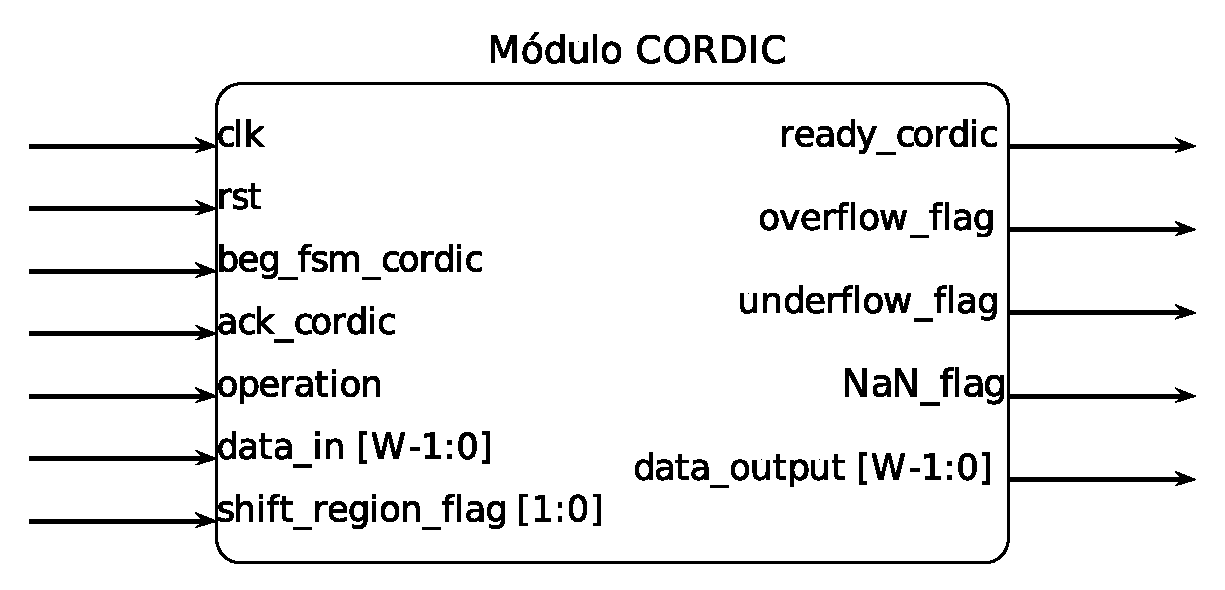
\includegraphics[width=0.7\textwidth]{CORDIC_Arch.eps}
  \caption{Diagrama de entradas y salidas para el módulo de calculo de seno, coseno y logaritmo natural, basado en el algoritmo CORDIC.}
  \label{fig:Cordic_Arch}
\end{figure}

Las señales de entrada del módulo son:

\begin{itemize}
\item	\textbf{clk:} reloj interno del sistema, con una frecuencia de 100 MHz, (Placa FPGA Artix-7 Nexys 4).
\item	\textbf{rst:} señal de reinicio de la máquina de estados finitos, o maquina de control, encargada de controlar el flujo de datos.
\item	\textbf{beg\_fsm\_cordic:} señal de inicio, que le indica a la máquina de control que se inicia el proceso para un nuevo cálculo de una de las operaciónes.
\item	\textbf{ack\_cordic:} señal proveniente de un sistema externo, y que le indica a la máquina de control que ha recibido el resultado de la operación de manera correcta.
\item	\textbf{operation:} señal de entrada que indica cuál operación se desea realizar. Esta codificación viene dada por la siguiente secuencia de bits:
\begin{itemize}
 \item	0: operación coseno.
 \item	1: operación seno.
\end{itemize}
\item	\textbf{data\_in:} señal de entrada, con un ancho de W bits, que contiene el valor del dato al que se desea realizar un cálculo, donde W puede tomar dos valores, 32 y 64, dependiendo de la precisión que se desea.
\item	\textbf{shift\_region\_flag:} señal de entrada utilizada en conjunto con las operaciones seno y coseno, que indica si el valor a calcular se encuentra en el segundo o tercer cuadrante. Esta codificación viene dada por la siguiente secuencia de bits:
\begin{itemize}
\item	00: El dato de entrada es un valor que se encuentra en el primer o cuarto cuadrante.
\item	01: El dato de entrada es un valor que se encuentra en el cuadrante.
\item	10: El dato de entrada es un valor que se encuentra en el cuadrante.
\item	11: El dato de entrada es un valor que se encuentra en el primer o cuarto cuadrante.
\end{itemize}
\end{itemize}


\subsection{Descripción del funcionamiento del Hardware CORDIC.}

En la Figura \ref{fig:Cordic_Arch_completa} se muestra el diagrama de bloques completo del Módulo CORDIC, en el cuál se muestran todas las etapas que conforman la arquitectura, implementada para la resolución de las operaciones seno, coseno y logaritmo natural, así como otras muchas más, las cuales se pueden implementar utilizando como base esta misma arquitectura, y realizando algunos cambios en cuanto a hardware y a la máquina de control.

En el diagrama se puede observar tanto los módulos por los cuales fluyen los datos, así como la máquina de estados y los contadores, que permiten controlar el flujo de los datos y controlar la cantidad de iteraciones realizadas, respectivamente. En la Figura \ref{fig:Cordic_Arch_completa} se observan señales con diferentes colores las cuales corresponden a:

\begin{itemize}
\item	Rojo: señal de reloj del sistema.
\item	Amarillo: señales de habilitación de los registros y los contadores.
\item	Verde: señal de reset de los registros de la arquitectura.
\item	Azul: señal de reset de la maquina de control.
\item	Negro: buses de datos.
\end{itemize}

\begin{figure}[H]
  \centering
  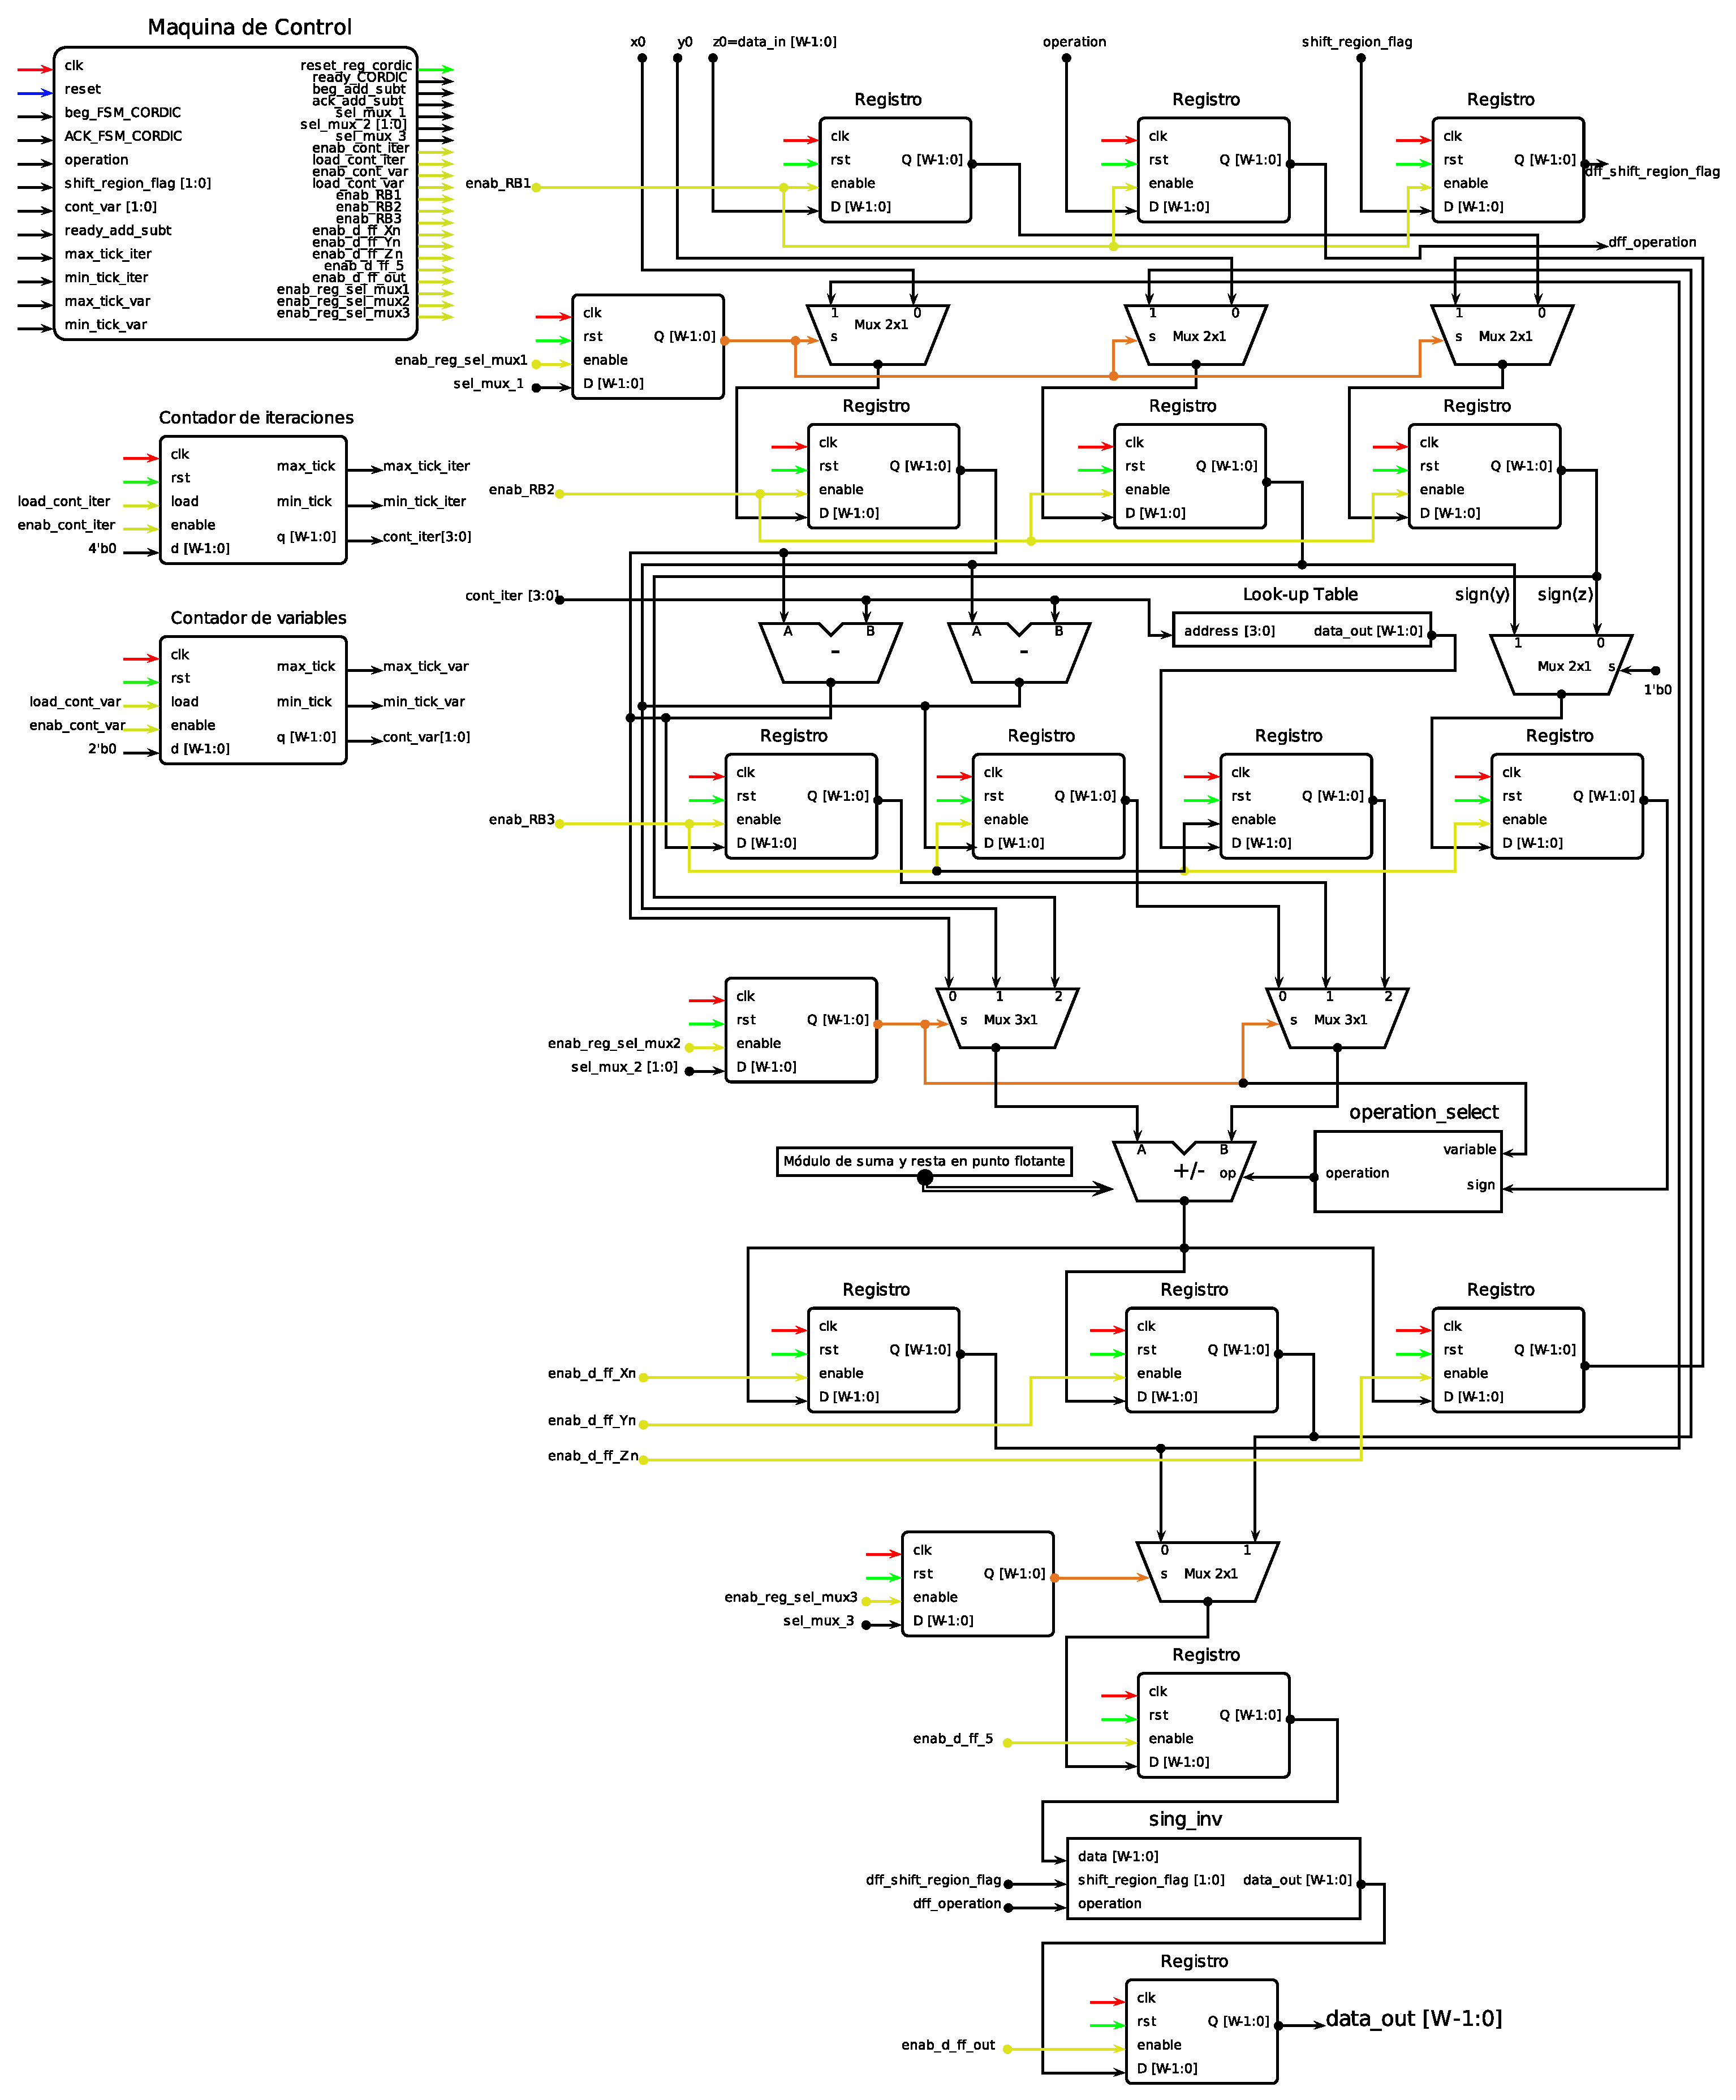
\includegraphics[width=1.1\textwidth]{cordic_completo.eps}
  \caption{Diagrama completo de la arquitectura CORDIC Bit-Paralela iterativa implementada junto con la maquina de control.}
  \label{fig:Cordic_Arch_completa}
\end{figure}

%------------------------------------------------------------------------------------------------------------------------------------

\newpage

Al ser el algoritmo \textit{CORDIC} un algoritmo iterativo, se debe tener en cuenta que entre más iteraciones se realicen, el porcentaje de error disminuye, pero esto conlleva a un mayor tiempo en la ejecución de la operación para obtener un resultado. Tomando en cuenta esta consideraciones, a continuación se explica detalladamente el funcionamiento del hardware implementado para la ejecución del algoritmo.

Al iniciar el proceso, se reciben 3 datos, los cuáles corresponden a las señales \textbf{operation}, $\textbf{shift\_region\_flag}$ y $\textbf{data\_in}$,  con tamaños de palabra de 1, 2 y \textbf{W} bits, donde \textbf{W} puede tomar los valores de 32 o 64, dependiendo de la precisión que se desee. Los valores de estas señales son guardados en los registros de entrada, que muestrean la señal de entrada cuando la señal de habilitación $\textbf{enab\_RB1}$ presenta un valor en alto. Las señales \textbf{x0} y \textbf{y0} que se observan en la Figura \ref{fig:Cordic_Arch_completa} corresponden a valores iniciales del algoritmo que son constantes, cuyos valores son:
\begin{itemize}
\item	\textbf{x0} = 0.607252935008881.
\item	\textbf{y0} = 0.
\end{itemize}

Después de que los valores iniciales son guardados en los registros, en la siguiente etapa, la máquina de control decide cuál de los dos canales de los 3 multiplexores debe ser habilitada. Para esto se verifica el valor de la señal $\textbf{min\_tick\_iter}$, proveniente del contador de iteraciones. 

Si ésta señal tiene un valor de 1 lógico, implica que se está realizando la primer iteración del proceso, por lo que el canal 0 de los multiplexores será habilitado, permitiendo así que los valores iniciales de las señales \textbf{x0}, \textbf{y0} y \textbf{z0}, la cuál corresponde a la señal de entrada $\textbf{data\_in}$, pasen a la siguiente etapa, que consiste en un conjunto de registros pipeline, que guardan el dato proveniente de las salidas de los multiplexores. En caso de que la iteración actual no se la primera, la señal $\textbf{min\_tick\_iter}$ tendrá un valor de 0 lógico, con lo que se activará el canal 1 de los multiplexores, y permitirá el paso de los valores de las variables \textbf{Xn}, \textbf{Yn} y \textbf{Zn}, calculados en la iteración anterior.

Una vez que los valores de salida de la primera linea de multiplexores han sido guardados en la segunda linea de registros pipeline, la siguiente etapa en el cálculo se encarga de 3 tareas:
\begin{itemize}
\item[1-]	Realizar la operación de desplazamiento sobre los valores de las variables \textbf{x} y \textbf{y}.
\item[2-]	Direccionar un valor en la salida de la ROM, dependiendo del valor de la iteración actual.
\item[3-]	Seleccionar entre el signo de la variable \textbf{y} o \textbf{z}, dependiendo del modo de operación del algoritmo.
\end{itemize}

En la Figura \ref{fig:etapa_desplaza}, se observa con mayor detalle las señales presentes en esta etapa y el ancho de palabra de cada una.

\begin{figure}[H]
  \centering
  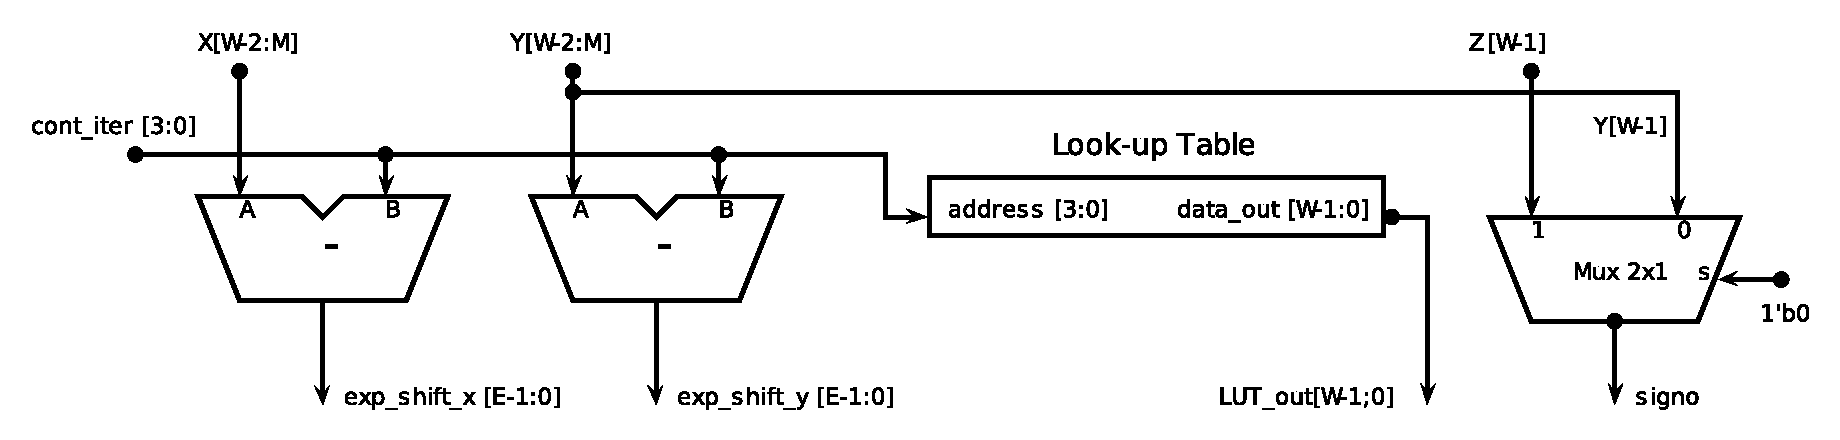
\includegraphics[width=0.75\textwidth]{etapa_desplaza.eps}
  \caption{Etapa de la Arquitectura \textit{CORDIC}, que realiza la operación de desplazamiento de las variables \textbf{x} y \textbf{y}, direcciona los valores de la ROM, y decide de cuál variable se toma el signo, dependiendo del modo de operación del algoritmo.}
  \label{fig:etapa_desplaza}
\end{figure}

En las Ecuaciones (\ref{eq:ec_rotacion}) del algoritmo \textit{CORDIC}, se observa que las variables $x_{i}$ y $y_{i}$, las cuáles corresponden a los valores obtenidos de las variables $X$ y $Y$ de la iteración anterior, son multiplicadas por el valor $2^{-i}$, que a nivel de hardware corresponde a la operación de desplazamiento a la derecha , $>>i$, donde $i$ es el valor de la iteración actual que se está realizando.

Pero debido a que se están utilizando valores en punto flotante, la operación de desplazamiento no consiste en insertar ceros a la derecha o izquierda del arreglo de bits. En cambio, si se desean hacer desplazamientos a la derecha , se realiza una resta, en la cuál al valor del exponente del arreglo de bits, se le resta el valor correspondiente a la cantidad de desplamientos a realizar, y si se desean hacer desplazamientos a la izquierda, se realiza una suma.

Por consiguiente, ya que en el algoritmo \textbf{CORDIC} se necesitan realizar desplazamientos a la derecha, se implementan dos restadores en punto fijo, que tienen como entradas las señales $X[W-2:M]$, $X[W-2:M]$ y $cont\_iter[3:0]$, tal como se muestra en la Figura \ref{fig:etapa_desplaza}, donde \textbf{W} representa el ancho de palabra, y \textbf{M} representa la cantidad de bits que ocupa la mantisa, por consiguiente, si se toma como ejemplo que el ancho de palabra de la arquitectura es \textbf{W}=32 bits, esto tendría como consecuencia que el valor de \textbf{M} sea 23, por lo que el ancho de palabra de las señales $X[W-2:M]$ y $X[W-2:M]$ es de 8 bits, y el rango que representa en el arreglo de bits es de [30:23], que son los bits que corresponden al campo de exponente en el arreglo.
 
En la salida de los restadores se obtiene como resultado un nuevo valor de exponente, con un ancho de palabra de $[E-1:0]$, donde \textbf{E} representa la cantidad de bits que ocupa el campo de exponente.

La siguiente tarea que se realiza en esta etapa consiste en direccionar un valor precargado en el módulo \textit{Look-up Table}, el cuál es una memoria ROM, que contiene los valores precalculados de la operación $arctan(2^{-i})$, donde como ya se ha explicado anteriormente, $i$ representa la iteración actual. Estos valores se utilizan para el cálculo de la variable $z_{i+1}$, presente en las Ecuaciones (\ref{eq:ec_rotacion}).

Por último, en ésta etapa se direcciona el bit de signo de las variables \textbf{Y} o \textbf{Z}, dependiendo del modo de operación del algoritmo \textit{CORDIC}. Como se observa en la Figura \ref{fig:etapa_desplaza}, esto se realiza mediante un multiplexor de 2 canales, que tiene como entradas el bit de signo de la variable \textbf{Z} en el canal 0, y el bit de signo de la variable \textbf{y}, en el canal 1.

Debido a que para el cálculo de las operaciones seno y coseno el algoritmo realiza los cálculo en el modo de rotación, y ya que estas son las dos operaciones implementadas en este proyecto, en la entrada de selección del multiplexor se coloca el valor constante de 0, que habilita el canal 0, direccionando a la salida el bit de signo de la variable \textbf{Z}.

Después de ser completadas estas tres tareas, las cuales se realizan en paralelo, los resultados son almacenados en un tercer conjunto de registros pipeline. Entre estos registros, cabe destacar los que guardan las variables \textbf{X} y \textbf{Y}, ya que a la entrada de estos registros, al bit de signo y los bit de mantisa de estas variables antes de ser desplazados se les concatena el nuevo valor de exponente, por lo que estos registros se utilizan para formar el patrón de bits correcto para las variables desplazadas en formato de punto flotante.

En la siguiente etapa, la cual se pueda observar con mejor detalle en la Figura \ref{fig:etapa_suma}, se procede a resolver cada una de las variables de las Ecuaciones (\ref{eq:ec_rotacion}). Primero, la máquina de control define cuál canal de los multiplexores se debe habilitar, teniendo en cuenta en cuál iteración pertenece el cálculo, si la operación es un seno o un coseno y a que región del plano cartesiano pertenece el ángulo a resolver.

\begin{figure}[H]
  \centering
  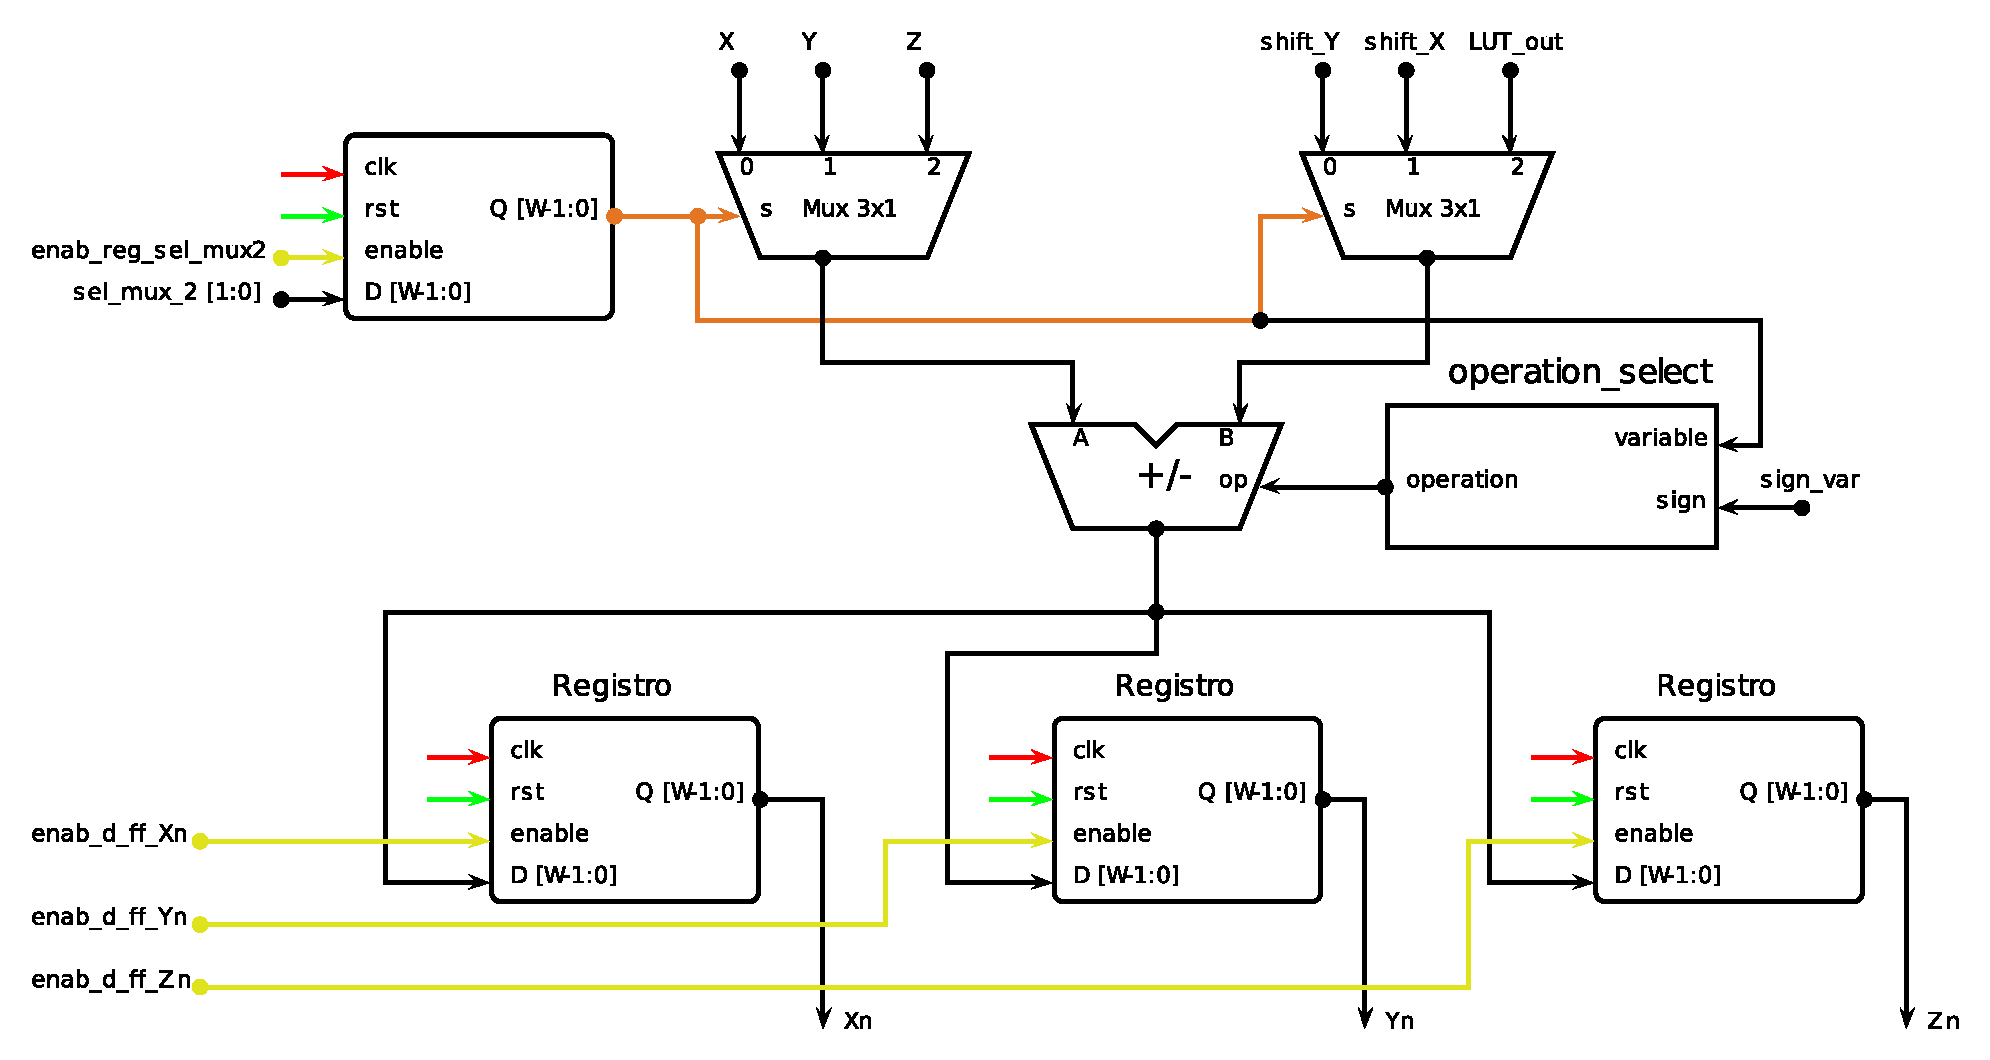
\includegraphics[width=0.75\textwidth]{suma_etapa.eps}
  \caption{Etapa de la Arquitectura \textit{CORDIC}, que realiza la suma o resta en punto flotante, dependiendo de cual variable se esté calculando y la iteración actual.}
  \label{fig:etapa_suma}
\end{figure}

Para entrar en más detalle, en caso de que se este realizando la última iteración, ya no se necesita realizar el cálculo de las tres variables, si no solo de una, ya sea de $X_{n}$ o $Y_{n}$, permitiendo con esto disminuir el tiempo que toma obtener un resultado final. Si la opeación a calcular es un coseno y el ángulo se encuentra en el $1^{er}$ o $4^{to}$ cuadrante del plano cartesiano, se activa el canal 0 de ambos multiplexores, con lo que permite el cálculo de la variable $X_{n}$.

En caso de que la operación a calcular es un seno, y al igual que en el caso anterior, sea la última iteración y el ángulo se encuentra en el $1^{er}$ o $4^{to}$ cuadrante del plano cartesiano, se activa el canal 1 de ambos multiplexores, con lo que permite el cálculo de la variable $Y_{n}$.

Ahora bien, si el ángulo más bien pertenece al $2^{do}$ o $3^{er}$ cuadarante, y al igual que los casos anteriores, se está realizando la última iteración, se intercambian los canales que se activan, esto quiere decir que en caso de que la operación sea un coseno, se activa el canal 1 y se calcula la variable $Y_{n}$, y si la operación es un seno, se activa el canal 0 y se calcula la variable  $X_{n}$.

Esto último permite al algoritmo \textit{CORDIC}, el cuál está limitado a realizar el cálculo de senos y cosenos en el rango de $[-90,90]$, poder ampliar el rango de cálculo a $[-180,180]$.

En caso de que no se este realizando la última iteración, es necesario realizar el cálculo de las tres variables, por lo que entra en juego el contador de variables, el cuál cuenta de 0 a 2, y la máquina de control se encarga de que el valor de salida del contador sea el que determine cual canal de los multiplexores se activa.

Por último, en esta etapa se encuentra el módulo $\textbf{operation\_select}$, el cuál decide si la operación a realizar es una suma o una resta. A partir de la Tabla \ref{Table:tabla_verdad_op}, la cuál es la tabla de verdad con la que se diseño el módulo, se observa que dicha tabla describe el funcionamiento de una compuerta \textit{XNOR}, cuyas entradas son el bit menos significativo de la señal de selección de los multiplexores de ésta etapa, y el bit de signo de la variable \textbf{Y} o \textbf{Z}, dependiendo del modo de operación en que se trabaje, en este caso de la variable \textbf{Z}.

\begin{table}[H]
\centering
\caption{Tabla de verdad que permite definir si se realiza una suma o resta en el módulo de suma/resta en punto flotante.}
\label{Table:tabla_verdad_op}
\begin{tabular}{|c|c|c|}
\hline
sel\_mux\_3 {[}0{]} & sign & operation \\ \hline
0                   & 0    & 1         \\ \hline
0                   & 1    & 0         \\ \hline
1                   & 0    & 0         \\ \hline
1                   & 1    & 1         \\ \hline
\end{tabular}
\end{table}

Una vez que el módulo de suma/resta en punto flotante brinda una solución, éstos valores son guardadados en 3 registros, los cuáles almacenan el valor de $X_{n}$, $Y_{n}$ o $Z_{n}$ dependiendo de cuál variable se estaba calculando. Cabe destacar que el módulo de suma/resta en punto flotante utilizado es el resultado de la propuesta de proyecto de graduación del compañero Francis López Montero.

La última etapa implementada en la arquitectura corresponde a la observada en la Figura \ref{fig:last_stage}, la cuál se encarga de  direccionar a la salida el valor de la variable $X_{n}$ o $Y_{n}$, e invierte el valor del bit de signo del resultado final, dependiendo de la operación y del cuadrante al que pertenesca el ańgulo a calcular.

\begin{figure}[H]
  \centering
  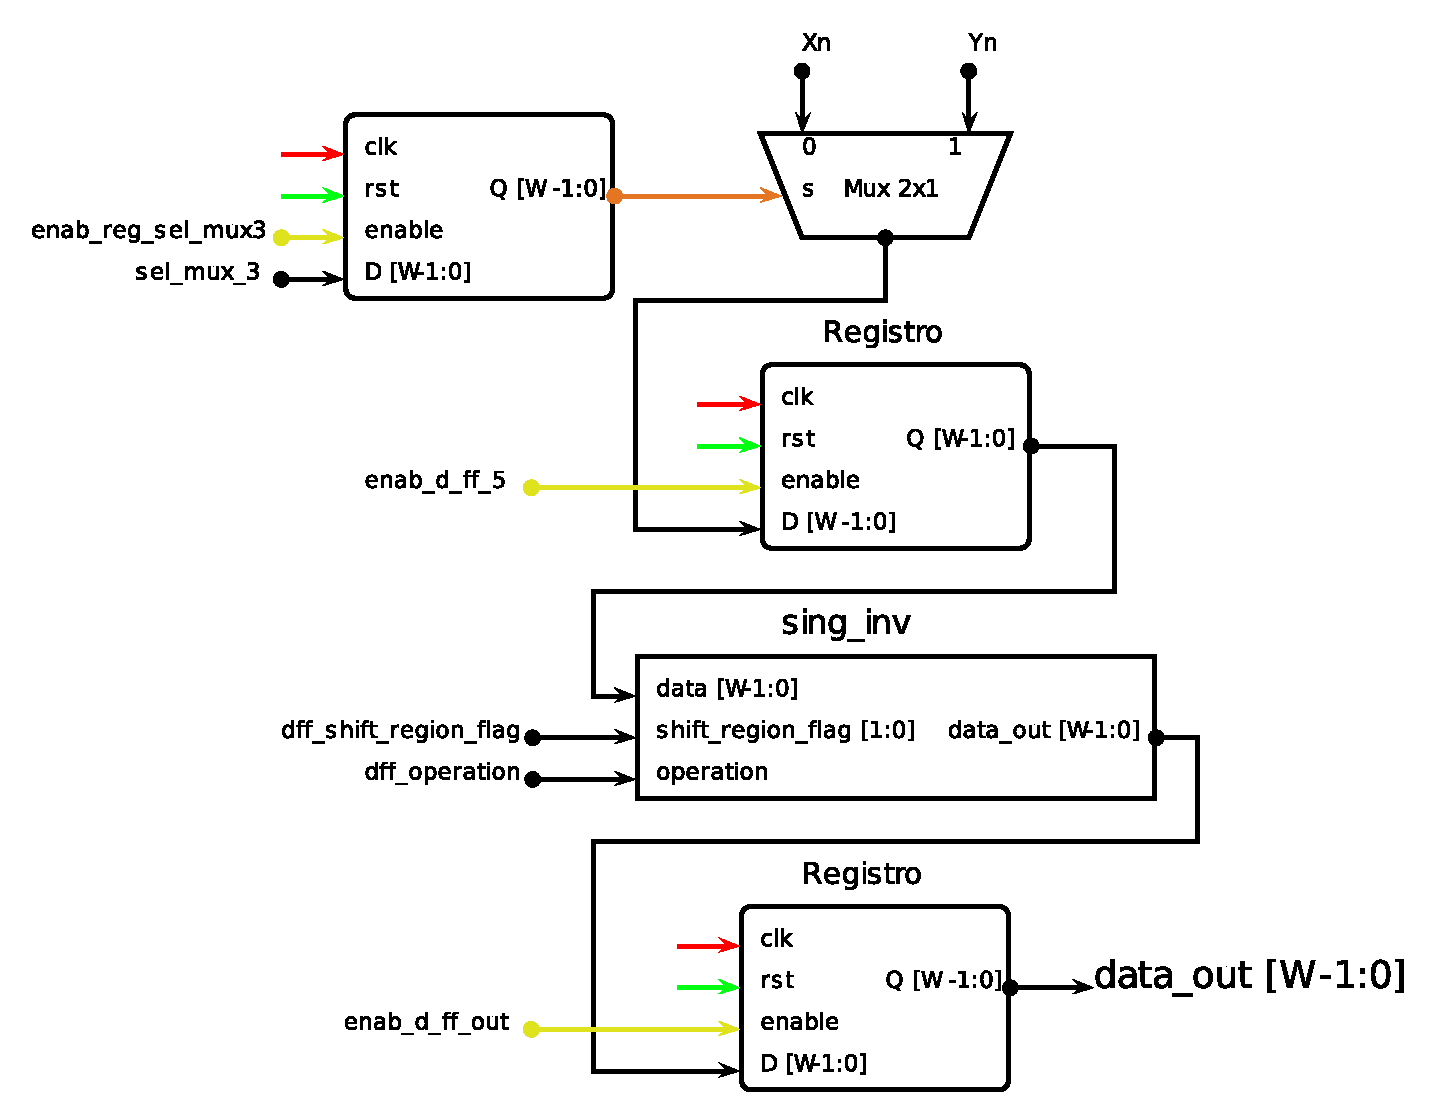
\includegraphics[width=0.75\textwidth]{last_stage.eps}
  \caption{Etapa de la Arquitectura \textit{CORDIC}, que direcciona a la salida el valor de la variable $X_{n}$ o $Y_{n}$, e invierte el valor del bit de signo, dependiendo de la operación y del cuadrante al que pertenesca el ańgulo a calcular.}
  \label{fig:last_stage}
\end{figure}


La señal de selección del multiplexor toma el valor de 0 lógico, permitiendo pasar a la salida el valor de la variable $X_{n}$,  en los siguientes casos:
\begin{itemize}
\item	La operación a calcular es un coseno y el ángulo a calcular pertenece al $1^{er}$ o $4^{to}$ cuadrante.
\item	La operación a calcular es un seno y el ángulo a calcular pertenece al $2^{do}$ o $3^{er}$ cuadrante.
\end{itemize}

En caso contrario, la de selección del multiplexor toma el valor de 1 lógico, permitiendo pasar a la salida el valor de la variable $Y_{n}$, en los siguientes casos:
\begin{itemize}
\item	La operación a calcular es un seno y el ángulo a calcular pertenece al $1^{er}$ o $4^{to}$ cuadrante.
\item	La operación a calcular es un coseno y el ángulo a calcular pertenece al $2^{do}$ o $3^{er}$ cuadrante.
\end{itemize}

Por último, el módulo \textbf{sign\_inv}, es el encargado de invertir el signo del resultado final en caso de que el ángulo a calcular se encuentre en el $2^{do}$ o $3^{er}$ cuadrante del plano cartesiano. Presenta las señales de entrada \textbf{data}, \textbf{shift\_region\_flag} y \textbf{operation}, las cuáles corresponde al resultado de la operación que se desea calcular, la señal que indica a que cuadrante del plano cartesiano pertence el ángulo a calcular y la señal que indica cual operación se realizó, respectivamente. 

La Tabla \ref{Table:tabla_verdad_signo}, es la tabla de verdad utilizada para diseñar el módulo \textbf{sign\_inv}, de esta manera se permite implementar este módulo en muy pocas lineas en el lenguaje \textit{Verilog}.

\begin{table}[H]
\centering
\caption{Tabla de verdad, utilizada para el diseño del módulo \textbf{sign\_inv}, encargado de cambiar el valor del bit de signo del resultado final, en los casos en que se necesite.}
\label{Table:tabla_verdad_signo}
\begin{tabular}{|c|c|c|c|c|}
\hline
operation & sign & shift\_region\_flag{[}1{]} & shift\_region\_flag{[}0{]} & new\_sign \\ \hline
0         & 0    & 0                          & 0                          & 0         \\ \hline
0         & 0    & 0                          & 1                          & 1         \\ \hline
0         & 0    & 1                          & 0                          & 0         \\ \hline
0         & 0    & 1                          & 1                          & 0         \\ \hline
0         & 1    & 0                          & 0                          & 1         \\ \hline
0         & 1    & 0                          & 1                          & 0         \\ \hline
0         & 1    & 1                          & 0                          & 1         \\ \hline
0         & 1    & 1                          & 1                          & 1         \\ \hline
1         & 0    & 0                          & 0                          & 0         \\ \hline
1         & 0    & 0                          & 1                          & 0         \\ \hline
1         & 0    & 1                          & 0                          & 1         \\ \hline
1         & 0    & 1                          & 1                          & 0         \\ \hline
1         & 1    & 0                          & 0                          & 1         \\ \hline
1         & 1    & 0                          & 1                          & 1         \\ \hline
1         & 1    & 1                          & 0                          & 0         \\ \hline
1         & 1    & 1                          & 1                          & 1         \\ \hline
\end{tabular}
\end{table}